This chapter describes the subjective view of the results derived from this thesis's program detailed in chapter three and four. Discussion about the results is elaborated upon in the following chapter.



\section{NPRA}
There are three levels of data available: monthly, weekly and hourly. For this reason, the monthly dataset will be disregarded as there are better data available. Weekly data distinctly show the Norwegian holidays described in table \ref{table:jesus} and shown in figure \ref{fig:graph_vacation_and_compare}. From the figure the Christmas holiday is shown in weeks 51 and 52, the easter holiday is distinctly shown at week 14 and ends at week 15, and week 25 to week 33 is the summer vacation. The dramatic drop at the end must be overlooked and may be explained as insufficient data (days) for that week. 

\begin{center}
\begin{table}[!h]
\begin{tabular}{ | m{9em} | m{10cm}| }
 \hline
 \textbf{Vacation/Holiday} & \textbf{When} \\ [0.5ex] 
 \hline
 Summer vacation & About nine weeks from the midth of June to the end of August  \\ 
 \hline 
 Autumn vacation & One week or a long weekend in September or October, usually in week 39, 40 or 41.\\ 
 \hline
 Christmas holiday & Usually two weeks from the end of December to the start of January\\ 
 \hline
 Winter vacation & Usually in week 7, 8 or nine in February or March \\ 
  \hline
 Easter holiday & 10-11 days at the end of March or beginning of April \\ 
  \hline
 Other and Christian holy days & Labour Day, Ascension Day, Constitution Day \\ 
  \hline
\end{tabular}
\caption{The Norwegian holidays and vacations}
 \label{table:jesus}
\end{table}
\end{center}

\begin{figure}[!htb]
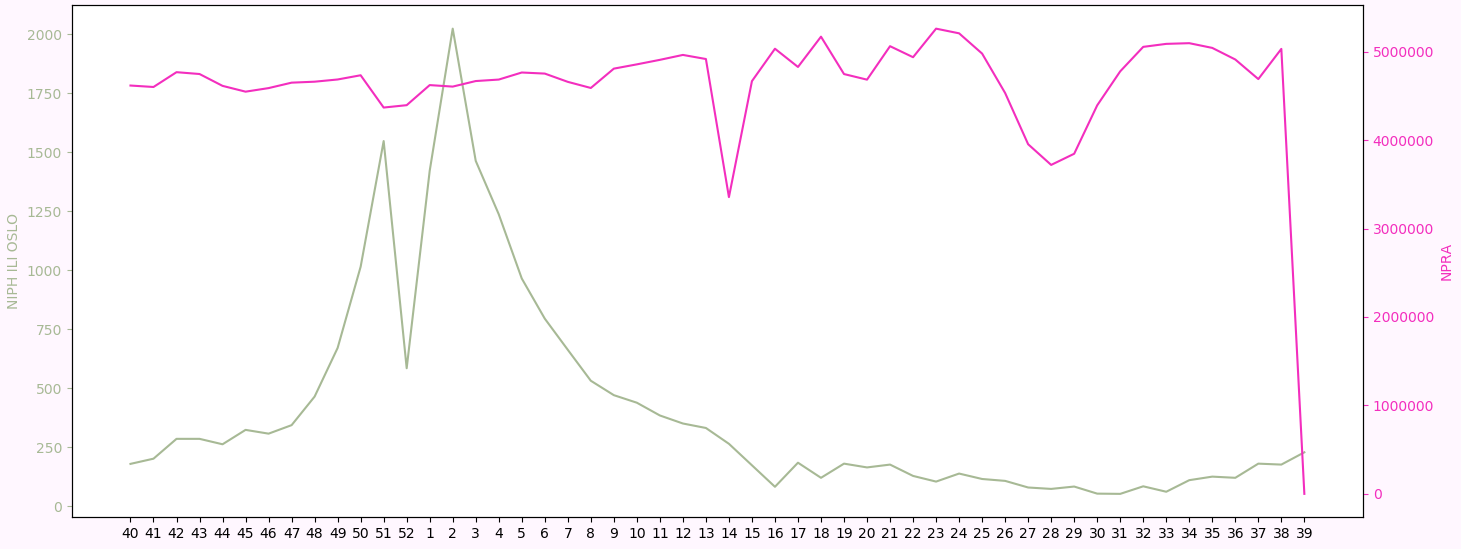
\includegraphics[width=16cm]{graph_vacation_and_compare}
\centering
\caption{NPRA data compared with the NIPH ILI data of the city of Oslo for the influenza season of 2016/2017}
\label{fig:graph_vacation_and_compare}
\end{figure}

It is important to take vacation and holidays into account when procuring information from these data, as otherwise, it would be easy to conclude wrongly. The most dramatic drop is the summer vacation, which luckily is outside the influenza season anyway. 

\newpage

Another challenge with holidays and vacations is that the start and duration change yearly, and because of the Gregorian calendar set dates shift one day up the next weekday for the next year, an exception is if there is a leap year, in that case, the shift is two days. This needs to be taken into consideration, and possibly weeded out or glossed over in order to avoid misinterpretations.
\\
Further, the weekly graphs show a considerable increase in traffic each year, when asked about this the NPRA admitted to their action plan to increase the numbers of traffic registration stations yearly. This increase of infrastructure is transparent in the graphs shown as jumps in the amount of traffic with each new year. From the end of November to the beginning of December there is a slight drop in the amount of traffic without there being any vacations or holidays, this anomaly might be correlated with the influenza season as numbers of reported virus observations and ILI incidents seems to increase at the same time. When the influenza season slowly begins to decline, traffic slightly returns to normal over the course of January to June. \\
The weekly data is an aggregated set of many traffic registration stations based on the cities of interest or the all of Norway, therefore roadworks, accidents or closed roads is not directly apparent. They are however visible, by assumption, on the hourly datasets as they only show one traffic registration station at a time. When in doubt of closed roads one could pick another traffic registration station nearby and see if it is also affected in the same manner. Another advantage with the hourly datasets is that there is not a dramatic yearly increase of traffic, which means more reliable data can be obtained, especially from the older traffic registration stations that have been operational for several years already.






\section{Twitter}
The way that twitter\_analyser.py works are that it simply counts the number of occurrences of tweets and then draws a graph based on that count. The Twitter data collected in twitter\_data.txt still contains duplicates although efforts were taken to prevent this. The duplicates may affect the graph drawn in batches as spikes where articles or hype are written about influenza or with other of the search terms. The Twitter data has a distinct pulse following the time when people post messages on social media the most by week\cite{socialTrend}, Mondays to Thursdays sees a high frequency of tweets, which decreases during the weekend. The relatively stable week-to-week distribution of tweets provides a baseline for social media behaviour patterns in relation to the flu. This at least shows that the data collected is somewhat in accordance with other social media in other parts of the world. During the collection of tweets the event of the Norwegian Easter holiday occurred, from the graph shown the spikes even out and there is a more consistent flow of tweets throughout the holiday.
When comparing the datasets of twitter and NIPH there is a clear similarity between them. The Twitter data seems to follow the trend downwards with the NIPH when the season is coming close to an end. However, the Twitter data seems to be lagging behind by 10 weeks, even less so with the ILI data from Bergen. This is in direct contradiction with both research referenced earlier in chapter two, and with this thesis's expectations. Figure \ref{fig:graph_twitter_ili_oslo} shows the comparison of Twitter data and NIPH ILI data from Oslo in this year's influenza season.

\begin{figure}[!htb]
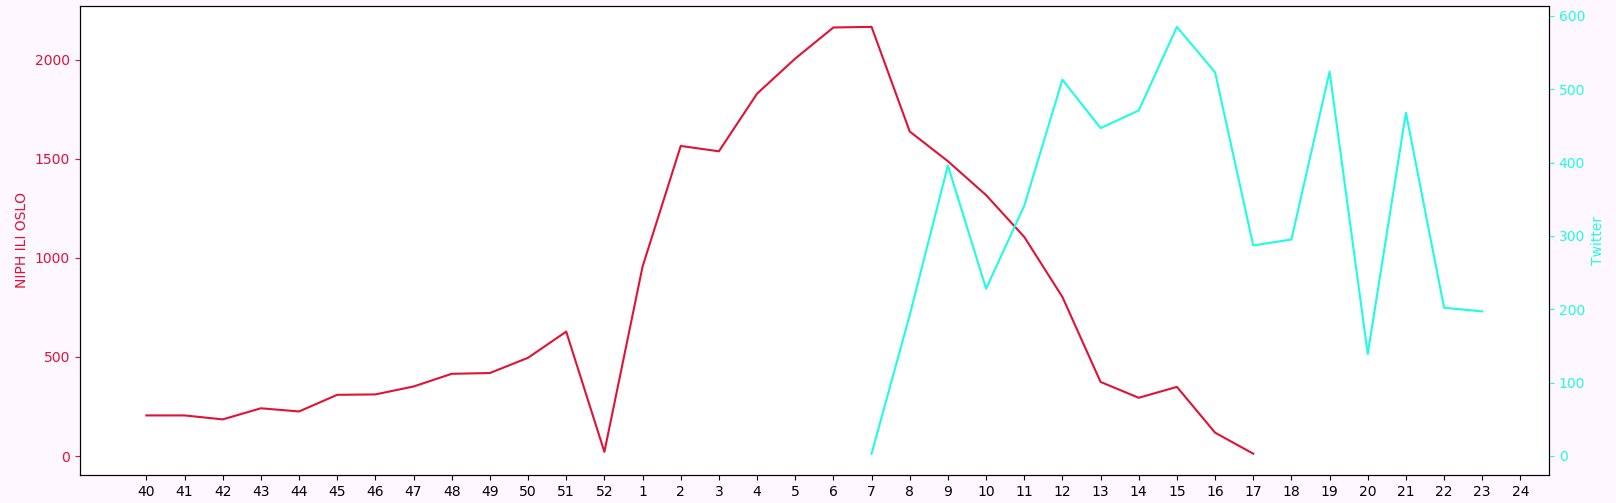
\includegraphics[width=16cm]{graph_twitter_ili_oslo}
\centering
\caption{Twitter data compared with the NIPH ILI data of the city of Oslo for the influenza season of 2017/2018}
\label{fig:graph_twitter_ili_oslo}
\end{figure}

TODO: si litt mer om grafen ...







\section{Kolumbus}
The Kolumbus data is the least interesting as it does not have spatial specific data and that the data resolution is too low on a monthly basis to see any anomalies. The longer Norwegian vacations and holidays are still somewhat visible though. This goes to show that sufficient temporal resolution is critical in order to derive any useful information from data in this thesis.




\section{Ruter}
Comparing the Ruter data with the ILI data of Oslo is especially interesting because Ruter is the public transportation administrator in that city. As with the NPRA data the Norwegian holidays and vacations are apparent as described in section 5.1. The weeks of 47, 48 and 49 show a slight decrease of passenger travel without overlapping any vacations and holidays, there is also a slight increase of reported ILI every influenza season in those weeks. Should this correlation be confirmed to be valid after further investigations, this represents a measure link between urban travel habits and presence of flu within a society.
After the Christmas holiday passenger travel struggle for a few weeks to 'catch up' to a more stable level, interestingly enough the influenza seasons usually are on its peaks at that very time.
The amount of passenger travel also seems to be slightly increasing as the influenza season declines.














